%----------------------------------------------------------------------------------
% Exemplo do uso da classe tcc.cls. Veja o arquivo .cls
% para mais detalhes e instruções.
%----------------------------------------------------------------------------------

% Seleção de idioma da monografia. Por enquanto as únicas opções
% suportadas são 'portuguese' e 'english'
% Para impressão em frente e verso, use a opção 'twoside'. Da
% mesma forma, use 'oneside' para impressão em um lado apenas.
\documentclass[portuguese,oneside]{tcc}

  %----------------------------------------------------------------
  % Coloque seus pacotes abaixo.
  %
  % Obs.: muitos pacotes de uso comum do LaTeX, como amsmath,
  % geometry e url já são automaticamente incluídos pela classe
  % (veja o arquivo .cls). Isso torna obrigatória a presença destes
  % no sistema para o uso desta classe, mas ao mesmo tempo o uso se
  % torna mais simples.  Recomendo a instalação da versão mais
  % recente da distribuição TeXLive (para Windows e UNIXes):
  % www.tug.org/texlive/
  %
  % Pacotes e opções já incluídas automaticamente:
  %
  % \RequirePackage[T1]{fontenc}[2005/09/27]
  % \RequirePackage[utf8x]{inputenc}[2008/03/30]
  % \RequirePackage[english,brazil]{babel}[2008/07/06]
  % \RequirePackage[a4paper]{geometry}[2010/09/12]
  % \RequirePackage{textcomp}[2005/09/27]
  % \RequirePackage{lmodern}[2009/10/30]
  % \RequirePackage{indentfirst}[1995/11/23]
  % \RequirePackage{setspace}[2000/12/01]
  % \RequirePackage{textcase}[2004/10/07]
  % \RequirePackage{float}[2001/11/08]
  % \RequirePackage{amsmath}[2000/07/18]
  % \RequirePackage{amssymb}[2009/06/22]
  % \RequirePackage{amsfonts}[2009/06/22]
  % \RequirePackage{url}
  % \RequirePackage[table]{xcolor}[2007/01/21]
  %----------------------------------------------------------------
  % Para inserção de figuras.
  \usepackage{graphicx}
  \usepackage{adjustbox}
  \usepackage{longtable}
  % Utilize a opção 'pdftex' se você estiver usando o pdflatex (que
  % permite figuras em formatos como .jpg ou .png)
  %\usepackage[pdftex]{graphicx}
  
  % Para tabelas com elementos ocupando mais de uma linha
  \usepackage{multirow}
  % Para frações na mesma linha (ex. ⅓).
  \usepackage{nicefrac}
  % Para inserir figuras lado a lado.
  \usepackage{subfigure}
  
  \usepackage{booktabs}
  % Para formatar algoritmos.
  % A opção [algo2e] é necessária para evitar conflitos
  % com as definições da classe.
  %\usepackage[algo2e]{algorithm2e}
  \usepackage{algorithmic}
  % Um float do tipo algoritmo. No momento
  % este pacote é incompatível com a classe.
  %\usepackage{algorithm}
  \usepackage{esint}
  %----------------------------------------------------------------
  % Autor (OBRIGATÓRIO)
  %----------------------------------------------------------------
  \author{Felipe Brizola Bergues Duro}
  
  %----------------------------------------------------------------
  % Título (OBRIGATÓRIO). Devem ser passados DOIS parâmetros,
  % o título em português E o inglês, não importando o idioma
  % escolhido. Os títulos são utilizados para a montagem da capa,
  % resumo e abstract mais tarde.
  %----------------------------------------------------------------
  \title{Mapeamento de recursos sob computação em névoa}
        {Mapping resources under the fog computing}
  
  %----------------------------------------------------------------
  % Opções para o tipo de trabalho (OBRIGATÓRIO)
  %----------------------------------------------------------------
  %\tipotrabalho{\ptci}         % Proposta de Trabalho de Conclusão
%   \tipotrabalho{\tci}         % Trabalho de Conclusão I
  \tipotrabalho{\tcii}        % Trabalho de Conclusão II
  
  %----------------------------------------------------------------
  % Seleção do curso ("este trabalho é um requisito parcial para
  % obtenção do grau de (mestre ou doutor) em Ciência da Computação").
  %----------------------------------------------------------------
  \curso{\cc} % Ciência da Computação
  %\curso{\si} % Sistemas de Informação
  %\curso{\es} % Engenharia de Software
  
  %----------------------------------------------------------------
  % Orientador (e Co-orientador, caso haja um). É OBRIGATÓRIO
  % informar pelo menos o orientador.
  %----------------------------------------------------------------
  \orientador{Prof. Dr. Sérgio Johann Filho}
  %\coorientador{Ciclano de Farias}
  
  %----------------------------------------------------------------
  % A capa é inserida automaticamente. Por isso não é necessário
  % chamar \maketitle
  %----------------------------------------------------------------
  \begin{document}
  
  %----------------------------------------------------------------
  % Depois da capa vem a dedicatória e a epígrafe.
  %----------------------------------------------------------------
  %  \dedicatoria{Dedicamos este trabalho a nossos pais. Sem eles, certamente, não teríamos a oportunidade de chegar até aqui. A educação que nos foi dada. com certeza, será para o resto da vida. }
  
  \epigrafe{Há três caminhos para o fracasso: não ensinar o que se sabe, não praticar o que se ensina, e não perguntar o que se ignora.} {São Beda}
  
  %----------------------------------------------------------------
  % Também dá para fazer as duas na mesma página:
  %----------------------------------------------------------------
  % \dedigrafe{Dedico este trabalho a meus pais.}
  %           {Just because something doesn’t do what you planned it to do doesn’t mean it’s useless.}
  %           {Thomas Edison}
  
  %----------------------------------------------------------------
  % A seguir, a página de agradecimentos (OPCIONAL):
  %----------------------------------------------------------------
  % \begin{agradecimentos}Agradeço a XYZ pessoas por...  \end{agradecimentos}
  
  %----------------------------------------------------------------
  % Resumo, com as palavras-chave passadas por parâmetro
  % (OBRIGATÓRIO, ao menos para teses e dissertações)
  %----------------------------------------------------------------
  %\begin{resumo}{mapeamento de recursos, computação em névoa, internet das coisas...}
  
  %Computação em névoa... .Este trabalho propõe desenvolver um protocolo no qual seja possível mapear recursos de dispositivos conectados a rede local....
  
  %\end{resumo}
  
  %----------------------------------------------------------------
  % Abstract, com as palavras-chave passadas por parâmetro
  % (OBRIGATÓRIO, ao menos para teses e dissertações)
  %----------------------------------------------------------------
  %\begin{abstract}{resource mapping, fog computing, internet of things...}
  %Traducao do resumo\end{abstract}
  
  %----------------------------------------------------------------
  % Listas e sumário, nessa ordem. Somente o sumário é obrigatório,
  % portanto, comente as outras listas, caso sejam desnecessárias.
  %----------------------------------------------------------------
  \listoffigures       % Lista de figuras      (OPCIONAL)
  \listoftables        % Lista de tabelas      (OPCIONAL)
  \listofalgorithms    % Lista de algoritmos   (OPCIONAL)
  \listofacronyms      % Lista de siglas       (OPCIONAL)
  %\listofabbreviations % Lista de abreviaturas (OPCIONAL)
  %\listofsymbols    % Lista de símbolos   (OPCIONAL)
  \tableofcontents     % Sumário               (OBRIGATÓRIO)
  
  %----------------------------------------------------------------
  % Aqui começa o desenvolvimento do trabalho. Para uma melhor
  % organização do documento, separe-o em arquivos,
  % um para cada capítulo. Para isso, utilize o comando \include,
  % como mostrado abaixo.
  %----------------------------------------------------------------
  %----------------------------------------------------------------------------------
% Exemplo do uso da classe tcc.cls. Veja o arquivo .cls
% para mais detalhes e instruções.
%----------------------------------------------------------------------------------
\chapter{\label{chap:intro}Introdução}

%%%%%%%%% TEM QUE ESTAR EM ORDEM ALFABETICA %%%%%%%%%%

%\sigla{CC}{Cloud Computing}

\sigla{BGP}{Border Gateway Protocol}
\sigla{IaaS}{Infrastructure as a Service}
\sigla{IP}{Internet Protocol}
\sigla{NIST}{National Institute of Standards and Technology}
\sigla{PaaS}{Platform as a Service}
\sigla{SaaS}{Software as a Service}
\sigla{TCC}{Trabalho de Conclusão de Curso}
\sigla{TCP}{Transmission Control Protocol}
\sigla{UDP}{User Datagram Protocol}

% Comando para inserir abreviaturas.
%
%\abrev{Abrev}{Abreviatura}
% \abrev{Inform}{Informática}
%
% Comando para inserir símbolos. Estes irão aparecer em ordem
% de ocorrência, já que o número da página está presente na lista
% de símbolos.
% \simbolo{Hz}{Hertz}
% \simbolo{$\pi$}{Constante com valor aproximado de $3.1415926$}%
%
% bom site sobre BRTs
%http://www.brtdata.org/location/latin_america/mexico/mexico_city
%

\section{Contextualização do problema}

A computação em nuvem tem sido amplamente adotada nos últimos anos por vários tipos de empresas, pois além de disponibilizar diversos tipos de modelos de serviços como SaaS, PaaS e IaaS, provê modelos de implantação de infraestrutura em nuvem privada, comunitária, publica e híbrida.

Ainda temos, segundo definição de computação em nuvem adotada pelo NIST\cite{Mell:2011}: "computação em nuvem é um modelo que permite acesso a um conjunto compartilhado de recursos computacionais configuráveis (por exemplo, redes, servidores, armazenamento, aplicativos e serviços) que podem ser provisionados e liberados  com um pequeno esforço de gerenciamento ou interação com provedor de acesso".
Essa flexibilidade, tanto de modelo de serviços quando nos modelos de implatações, pode justificar o aumento no emprego desse modelo de computação.

Como a computação em nuvem não é Panacéia\footnote{Mecanismos ou práticas que, hipoteticamente, são capazes de solucionar os problemas e/ou dificuldades.}, podemos utilizar a definição de  Bonomi, Milito, Zhu e Addepalli\cite{Bonomi:2012} que diz: "a computação em nuvem libera as empresas e os usuários finais de muitos detalhes de especificações. Essa facilidade torna-se um problema para aplicações sensíveis à latência, que requerem que nós próximos atendam suas necessidades de forma eficiente". 
Como a interação entre os nós e os servidores na nuvem ocorrem através da internet, a baixa latência torna-se indispensável para aplicações que requerem eficiência na comunicação entre nós (por exemplo Robôs, drones, e carros de autônomos).
Portanto há uma lacuna entre aplicações que já utilizam modelos de computação em nuvem e aplicações que necessitam de baixa latência de rede e comunicação entre nós próximos, e é nesse hiato que a computação em névoa surge.

A computação em névoa é um assunto relativamente novo e teve sua primeira definição, dada pela cisco 2012, como uma extensão do paradigma de computação em nuvem provendo armazenamento, computação e serviços de rede entre dispositivos finais e os servidores na nuvem\cite{DBLP:journals/corr/RomanLM16}.

Atualmente a computação em névoa tornou-se um paradigma próprio e não mais uma mera extensão da computação em nuvem.
Esse paradigma criou o conceito de fog nodes que abrangem desde dispositivos finais com baixa capacidade computacional até servidores poderosos na nuvem. Assim, os fog nodes passam a fazer parte da implementação dos serviços em nuvem.
O que torna a computação em névoa interessante é a capacidade dessa variedade de dispositivos cooperarem uns com os outros de forma distribuída.
Temos, então, a névoa como uma arquitetura de três camadas (clientes <-> fog nodes <-> servidores centrais) na qual os servidores centrais podem coexistir com os fog nodes, todavia esses servidores não são essenciais para a execução dos serviços em névoa \cite{DBLP:journals/corr/RomanLM16}.

\section{Motivação e justificativa}

Descoberta e sincronização, computação e limite de armazenamento, gerenciamento, segurança, padronização, monetização e programabilidade serão os sete desafios que a computação em névoa deverá enfrentar para tornar-se realidade, segundo Vaquero e Rodero-Merino\cite{Vaquero:2014}.

Padronização, descoberta e sincronização serão os desafios explorados neste trabalho, pois hoje não há mecanismos padronizados no qual um membro da rede, seja ele uma raspberry-pi gerenciando sensores ou um computador, anuncie seus recursos ou consuma informações de outros nodos.

\section{Objetivo}
                                                                                                                        
Partindo do pressuposto de que cada nodo desta névoa estará executando um middleware que gerencie seus recursos locais, o objetivo principal deste trabalho de conclusão é construir um protocolo de rede que seja capaz de: descobrir, sincronizar e utilizar recursos de nodos em uma rede sob computação em névoa.       



% Lapidar esse exemplo.
% Imagem ilustrando fog
%Exemplificando uma aplicação em névoa podemos imaginar o seguinte cenário: sensores no alto dos postes de luz capazes de detectar luzes de emergencia de ambulâncias.
%Estes sensores enviam dados para um “fog node”.
%Os semáforos desta cidade podem sem abertos ou fechados remotamente. 
%Enquanto a ambulância estiver em deslocamento, os sensores dos postes podem enviar dados para o “fog node”, e este deve acionar os semáforos que estiverem na rota da ambulância. Por fim, quando a ambulância chegar ao hospital o fog node de lá pode enviar os dados para a nuvem.
%Imaginando que todo fog node é um dispositivo com conexão LAN(Local Area Network) e que precisa interagir com seus nós próximos



 
 
 
 
 
 
 
 








 %intro
  \chapter{\label{chap:chap2} Fundamentação Teórica}

Este capítulo apresentará alguns protocolos de comunicação que servirão de apoio para o desenvolvimento deste TCC. 
Por fim, alguns trabalhos relacionados a área serão expostos, bem como o posicionamento deste perante aos demais.

\section{Taxonomias em Arquiteturas de Computadores}
% -Taxonomias em Arquiteturas de Computadores (FLYNN - taxonomia, TANENBAUM, A. Organização estruturada de computadores)
\section{Máquinas multiprocessadas}
% -Máquinas multiprocessadas / paralelismo
\section{Modelos para troca de mensagens em aplicações}
% -Modelos para troca de mensagens em aplicações: cliente/servidor (sockets, RPC, RMI, MPI...), Publish/Subscribe, Webservices, Microservices 


\section{Protocolos relacionados}

\subsection{CoAP}

Especificado pela RFC-7252, o CoAP, protocolo de aplicação restrita, foi projetado para aplicações máquina-a-máquina
e tem como foco a transferência de documentos web entre nodos com recursos limitados em redes de baixa qualidade\cite{rfc7252}.

O modelo de interação cliente/servidor é o padrão adotado pelo CoAP, entretanto,
o fato do protocolo ter sido projetado para aplicações máquina-a-máquina faz com que os dispositivos comumente desempenhem o papel de cliente e servidor simultaneamente.

Quando mensagens CoAP de requisição e resposta são trocadas, estas devem conter o código do método ou código da resposta, respectivamente.
Além dos códigos, as mensagens podem conter outras informações, como o recurso que se deseja acessar e o tipo de mídia que se está transportando.
Por fim, um token é utilizado para que haja a correspondência entre requisição e resposta.

A Figura \ref{fig:fig4} ilustra uma solicitação entre cliente e servidor, na qual o cliente deseja obter a temperatura medida pelo sensor atrelado ao servidor.
Analisando a troca de mensagens, notamos que o cliente envia uma solicitação não confirmável com token 0x74 e código GET para acessar o recurso temperatura no servidor.
O servidor por sua vez retorna o código de resposta 2.05, que indica sucesso, o mesmo token que recebeu na solicitação do cliente e o valor 22.5 C.

\begin{figure}[htb!]
    \centering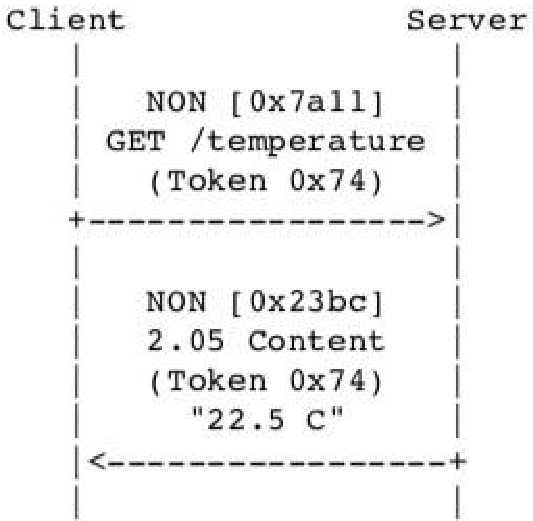
\includegraphics[height=.4\textwidth]{fig4.png} 
    \caption
    {\label{fig:fig4} Requisição e resposta utilizando mensagens não confirmáveis.} \cite{rfc7252}
\end{figure}

A arquitetura REST, assim como no protocolo HTTP\cite{rfc2616}, foi utilizada na projetização do protocolo CoAP.
Como ambos compartilham da mesma arquitetura, realizar o mapeamento de HTTP para CoAP e vice-versa é bastante simples.
Para realizar tal mapeamento basta utilizarmos o \textit{cross-proxy}, definido na seção 10 da própria RFC-7252\cite{rfc7252},
que converte o método ou tipo de resposta, tipo de mídia e opções para os valores HTTP correspondentes.

Além do modelo de comunicação cliente/servidor e da arquitetura REST, o CoAP também dispõem de outros princípios comuns ao HTTP e que são conceitos padrão na web,
como suporte a URIs\cite{rfc3986} e tipos de mídia da Internet(MIME)\cite{rfc2046}.

Entre o HTTP e CoaP nem tudo são semelhanças, pois, obviamente, este possui particularidades para que consiga atender aos requisitos no qual se propõe a resolver.
Entre as diferenças está a troca de mensagens assíncronas utilizando transporte orientado a datagramas, como UDP.
Apesar de, naturalmente, o protocolo UDP não prover confiabilidade, no CoAP é possível definir que as mensagens possuam tal aspecto.

\textit{Constrained RESTful Environments (CoRE) Link Format}, que será abordado na seção a seguir, possibilidade de envio de solicitações multicast e unicast, \textit{service discovery}, cabeçalho com baixa sobrecarga de dados e segurança na forma de DTLS\cite{rfc6347}
estão entre as principais caracteristicas do protocolo de aplicação restrita, CoAP.

\subsection{Constrained RESTful Environments (CoRE) Link Format}

Segundo a RFC-6690, a finalidade desta especificação é realizar REST em nodos com recursos limitados, sendo tal característica importante em aplicações maquina-a-maquina\cite{rfc6690}.
Em aplicação deste tipo é primordial que as configurações não dependam de interação de humanos, portanto, devem manter seu funcionamento sem configurações estáticas.


A principal função desta especificação é fornecer identificadores, denominados URIs, para os recursos hospedados em servidores. 
Para além, é possível que essas URIs possuam atributos relacionados aos recursos.
Estes atributos dividem-se basicamente em dois: rt, \textit{resource type} e if \textit{interface description}.
O primeiro é utilizado para para atribuir um nome que descreva de forma clara e enxuta um recurso,
já o segundo tem por objetivo indicar a interface especifica que interagirá com o recurso destino.

Um aspecto relevante ao CoRE, e de suma importancia para aplicações maquina-a-maquina, é o fato de possuir como URI padrão o prefixo \textit{/.well-known/core} , definido na RFC-5785\cite{rfc5785}.
Este prefixo é utilizado para que o servidor exponha suas políticas e recursos disponíveis.

O protocolo CoAP prevê suporte à CoRE e ao prefixo \textit{/.well-known/core}.
Contando com esses suportes, é possível traçarmos uma pequena analogia entre a arquitetura REST e o protocolo CoAP, pois tanto em REST quanto em CoAP, as URIs são utilizadas para a identificação de recursos.
Sendo assim, servidores CoAP ficam aguardando por requisições que utilizem tal URIs.

Para exemplificarmos, abaixo está um ciclo de requisição e resposta entre um cliente e um servidor com nomenclatura \textit{example.net}.
Este cliente deseja saber as políticas e recurso disponíveis pelo servidor, e para tal utiliza o prefixo padrão \textit{/.well-known/core}.

\begin{verbatim}
    REQ: GET coap://example.net/.well-known/core
\end{verbatim}

\begin{verbatim}
    RES: 2.05 Content
        </sensors/temp>;if="sensor",
        </sensors/light>;if="sensor"
\end{verbatim}


Analisando a resposta é fácil notar que este servidor possui dois recursos disponíveis,
sendo ambos com interface do tipo sensor, porém, um utilizado para medir temperatura e outro para medir intensidade de luz.
Juntamente aos dados, o codigo 2.05 é retornado indicando que a operação transcorreu com sucesso.

\subsection{MQTT - Message Queue Telemetry Transport}

O protocolo MQTT, inicialmente desenvolvido pela IBM, tornou-se um padrão para aplicações de IoT, pois mostrou-se escalável em ambientes com redes instáveis.
Essa caracteristica dá-se pelo fato do protocolo implementar um modelo asíncrono de troca de mensagens, deste modo, o emissor mantém-se desacoplado do receptor.
Diferentemente de um modelo cliente/servidor, HTTP por exemplo, o protocolo faz uso da técnica \textit{publish/subscribe}.


Essa técnica requer a existência de duas entidades, clientes e ao menos uma entidade central denominada \textit{broker}.
O funcionamento básico do protocolo em questão é demonstrado em três passos.

\begin{itemize}
    \item O cliente pode assinar qualquer tópico de mensagens no broker, e para tal precisa conectar-se a ele. Essa conexão pode ser uma conexão TCP/IP simples ou uma conexão TLS criptografada para mensagens sensíveis.
    \item O cliente publica as mensagens em um tópico do broker.
    \item Em seguida, o broker encaminha a mensagem a todos os clientes que assinam esse tópico.
\end{itemize}

Baseado nas caracteristicas descritas, notamos que o protocolo necessita de um ponto central de comunicação entre os nodos do sistema.
Neste caso o broker faz com que o MQTT seja um protocolo centralizado, pois, caso ele fique inoperante toda a rede MQTT passa a ficar desatualizada.

\section{Trabalhos Relacionados}

Spencer Lewson implementou um protocolo em nível de aplicação \cite{tanenbaum2011redes} capaz de realizar a comunicação entre nodos sob computação em névoa.
A especificação do protocolo e um \textit{middleware} capaz de realizar o gerenciamento dos recursos dos dispositivos, são os principais componentes deste trabalho \cite{Spencer:2015}.

Sua implementação requer que haja um ponto central de comunicação entre os nodos, uma vez que a conectividade entre eles ocorre via \textit{Bluetooth LE}.
A existência desse ponto justifica-se pelas regras de implementação do \textit{Bluetooth LE}, na qual descreve dispositivos de duas naturezas: centrais e periféricos.
Dispositivos centrais são responsáveis por descobrir dispositivos periféricos que estão interessados em criar conexão.
Portanto, a característica do \textit{Bluetooth LE} faz com que a topologia de rede e a arquitetura do projeto não seja distribuída \cite{Spencer:2015}.

A plataforma Iotivity \cite{iotivity}, mantida pela Linux Foundation, tem como cerne a criação de um padrão no qual os dispositivos conectam-se entre si e a Internet.
Esta plataforma possui quatro funcionalidades chaves, sendo elas, descoberta de recursos, gerenciamento de dados e dispositivos e transmissão de dados.

Focaremos na descoberta de recursos providos pela plataforma, pois, é o item que mais se assemelha a proposta deste trabalho de conclusão.
Como primeiro passo para a execução desta funcionalidade, devemos registrar o recurso utilizando sua URI e IP.
Após o registro, é possível especificarmos que este recurso é observável, ou seja, quando houver algum evento o nodo que o registrou como observável será notificado.
Apesar da plataforma Iotivity possuir outras funcionalidades, ela não possui mecanismos para manter o mapeamento de recursos em redes locais.

\begin{table}[htb!]
    \centering
    \caption{Comparação de funcionalidades.}
    \begin{tabular}{|l|c|c|c|c|c|}
    \hline
                                   & CoAP  & S. Lewson & Iotivity & MQTT  & Protocolo proposto \\ \hline
    Complexidade                   & média & média     & alta     & baixa & baixa              \\ \hline
    Bluetooth                      & não   & sim       & sim      & sim   & não                \\ \hline
    Lan                            & sim   & sim       & sim      & sim   & sim                \\ \hline
    Internet                       & sim   & não       & sim      & sim   & não                \\ \hline
    Map. de recursos               & sim   & sim       & sim      & sim   & sim                \\ \hline
    Sincronização do map.          & não   & não       & não      & não   & sim                \\ \hline
    Recursos observáveis           & n/a   & n/a       & sim      & sim   & não                \\ \hline
    Distribuído                    & não   & não       & não      & não   & sim                \\ \hline
    \end{tabular}
    \label{table:tab1}
\end{table}
 %ref teorico. estado da arte
  \chapter{\label{chap:chap3} Proposta de trabalho}

Seguindo a organização arquitetural da Figura \ref{fig:fig1}, a proposta deste trabalho é fazer com que um \textit{fog node} conheça, de forma autônoma, os recursos disponibilizados por seus vizinhos.
Assim, cada \textit{fog node} saberá quais são os \textit{edge devices} disponíveis na rede, portanto,
o nodo que possui o sensor de chuva saberia que existe um outro nodo na rede capaz de medir a temperatura, por exemplo.


Podemos observar na topologia da Figura \ref{fig:fig1}, que os \textit{fog nodes} não possuem uma um nodo central como servidor.
Em razão da topologia distribuída, se for necessário escalarmos a quantidade de nodos na rede, a mesma não deverá sofrer impactos significativos de performance.

Nas seções a seguir abordaremos a arquitetura, módulos e submódulos que compõem o projeto, bem como resultados esperados, validações e cenários de teste. 

\section{Arquitetura}

Esta Seção define a pilha de protocolos a serem utilizados neste projeto, bem como a justifica pela escolha dos mesmos.
A pilha de protocolos atuará em conjunto com a organização arquitetural previamente definida na Figura \ref{fig:fig1}.

A fim de facilitar a compreensão da arquitetura deste projeto, a Figura \ref{fig:fig2} explicita a pilha de protocolos que o projeto fará uso para implementar as funcionalidades propostas.

\begin{figure}[htb!]
    \centering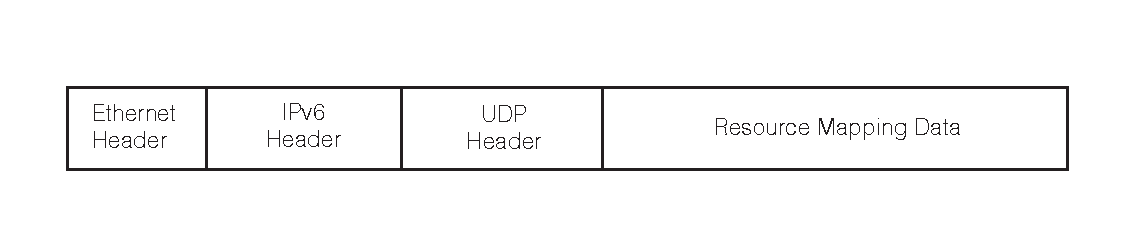
\includegraphics[width=.5\textwidth]{fig2.pdf}
    \caption%[This figure has a shorter caption now]%
    {\label{fig:fig2} Pilha de protocolos.}
\end{figure}

O modelo de referência TCP/IP é constituido de cinco camadas: física, enlace, rede, transporte e aplicação \cite{tanenbaum2011redes}.
Nesse trabalho, o níveis de rede e transporte (IPv4 e UDP respectivamente) serão utilizados para a implementação do modelo proposto.

A utilização de IPv4 na camada de rede justifica-se pelo fato do protocolo ser empregado em redes locais, que geralmente não necessitam de uma quantidade de endereçamento tão grande 
se comparado ao IPv6, mas não existem impedimentos para que implementações futuras utilizem IPv6 na camada de rede.

Manter o contexto de conexão entre os nodos, utilizando TCP por exemplo, despenderia uma quantidade de trafego desnecessário na rede.
Visto que a simplicidade é um dos objetivos deste trabalho e que transitar uma pequena quantidade de dados a cada requisição aumenta o desempenho da solução,
a utilização de datagramas UDP faz sentido neste protocolo

O protocolo proposto, entitulado \textit{Resource Mapping}, como apresentado na Figura \ref{fig:fig2}, atuará na camada de aplicação do modelo de referência TCP/IP \cite{tanenbaum2011redes} e será responsável por padronizar, descobrir e sincronizar os nodos da névoa.
Os maiores desafios neste modelo proposto são manter o estado global dos recursos acessível a todos os nodos, e garantir que o desempenho seja satisfatório com o objetivo permitir a escalabilidade da solução.



\section{Módulos}

De forma geral, cada nodo da rede deverá manter uma lista com os endereços IP`s que fazem parte do mapeamento.
Atrelado à cada endereço IP, deverá haver uma lista com os recursos providos por este.
Em vista disso, cada nodo portará um mapeamento global de recursos disponíveis na névoa.

% SJF: Podes dar a dica aqui (sem entrar em maiores detalhes) de que o mapeamento de recursos será atualizado sob demanda o que implicará em uma menor necessidade de tráfego para manter o estado global atualizado e permitirá uma maior escalabilidade de nodos / recursos.

O detalhamento das funcionalides que o projeto deverá dispor, bem como ilustrações relacionadas aos fluxos, serão abordadas nas proximas subseções.

\subsection{Middleware}

Observando a Figura \ref{fig:fig1}, notamos que há comunicação entre um fog node e seus respectivos edge devices.
A comunicação entre estes não é o foco deste projeto, portanto, será tratada de forma simulada.
Assim sendo, a simulação deverá prever alguns casos que, por vezes, possam suceder. Dentre alguns dos eventos possíveis está
o acréscimo ou remoção de um edge device vinculado à algum fog node.

A manutenção dos recursos, acréscimo ou remoção, transcorrerá utilizando o protocolo CoAP.
Utilizar CoAP para estas funcionalidades faz sentido, uma vez que este prevê meios para vinculação de recursos a nodos.

Segundo a definição de POST do protocolo CoAP, sua função é determinada pelo servidor que está recebendo a requisição e pelo do recurso referenciado na URI.
Geralmente a sua utilização resulta na criação ou atualização de um recurso.\cite{rfc7252}.
Já a mesma RFC define o método DELETE como sendo um método de remoção de recursos baseado em URIs\cite{rfc7252}.

Nessa perspectiva, portanto, o uso do método POST faz sentido para gerarmos \textit{(CoRE) Link Format} e o método DELETE para removermos.


\subsection{Descoberta de recursos}


Partindo do pressuposto que os nodos da névoa já possuem seus recursos devidamente criados e acessíveis via CoAP,
como primeiro passo do mapeamento devemos considerar a entrada de um novo nodo na rede.
No momento em que o nodo dispor de um endereço IP válido, este deverá enviar um pacote para o endereço de broadcast indicando que possui recursos a serem disponibilizados.


Ao receberem o pacote enviado por broadcast, os nodos que desejarem saber quais recursos estão sendo providos por este novo membro, deverão realizar uma query
unicast para a URI \textit{/.well-known/core} utilizando o protocolo CoAP.
Vale lembrar que este fluxo de requisição e resposta, utilizando a URI \textit{/.well-known/core}, faz com que o nodo requisitado retorne todos seus recursos ao solicitante.


Com o objetivo de exemplificar a primeira fase do protocolo, as Figuras \ref{fig:fig5} e \ref{fig:fig6} apresentam o fluxo para a descoberta de recursos.

%  mencionar q cada fog tem edge devices
A topologia da névoa utilizada nas imagens é definida por fog nodes enumerados de um à cinco, sendo o nodo FN5 o ultimo a entrar na rede.
A figura \ref{fig:fig5} demonstra o nodo FN5 entrando na névoa e, portanto, deverá anunciar-se por broadcast indicando que possui recursos a serem disponibilizados.

\begin{figure}[htb!]
    \centering\includegraphics[width=.5\textwidth]{fig5.png}
    \caption%[This figure has a shorter caption now]%
    {\label{fig:fig5} Nodo entrando na névoa.}
\end{figure}

Após FN5 enviar mensagem  “Hello“ por broadcast, os nodos FN1, FN2 e FN4 realizam a query diretamente ao FN5 afim de obter os recuros disponíbilizados por ele,
já o nodo FN3, por não estar executando o protocolo de mapeamento, não.


\begin{figure}[htb!]
    \centering\includegraphics[width=.5\textwidth]{fig6.png}
    \caption%[This figure has a shorter caption now]%
    {\label{fig:fig6} Nodos realizando query.}
\end{figure}


\subsection{Gerenciamento de recursos}

A manutenibilidade da lista de recursos globais é relevante para que a implementação do protocolo tenha sucesso, pois, a névoa deverá saber quando um nodo, ou recurso dele, deixou de fazer parte rede.
Para tal, faz-se necessário a utilização de alguns mecanismos de controle.
Esses controles são realizados em duas esferas, a primeira trata da inserção ou remoção de um nodo na rede,
já a segunda refere-se a inserção ou remoção de um edge device, vinculado a um nodo qualquer.
% SJF: Ta um pouco confuso esse parágrafo. Tenta remover as vírgulas, reescrevendo e mudando um pouco o estilo.



Inicialmente abordaremos a entrada e saída de nodos da névoa, e para esta subseção será utilizado o cenário da Figura \ref{fig:fig6} quando necessário.
O Pseudocódigo \ref{alg:alg1} demonstra, de forma sucinta, a política de atualização que cada nodo deverá implementar.

\begin{algorithm}[htb]
    \begin{center}
        \begin{algorithmic}[1]
            \STATE \textbf{function} $\text{Police(ip, resources)}$
            \STATE \hspace{\algorithmicindent} \textbf{if} $\text{exists(ip)}$
            \STATE \hspace{\algorithmicindent} \hspace{\algorithmicindent} $\text{update(ip, resources)};$
            \STATE \hspace{\algorithmicindent} \textbf{else}
            \STATE \hspace{\algorithmicindent} \hspace{\algorithmicindent} $\text{insert(ip, resources)};$
        \end{algorithmic}
    \end{center}
    \caption[Política de atualização de recursos]%
        {\label{alg:alg1} Política de atualização de recursos.}%
    \end{algorithm}

No momento em que o nodo recebe a resposta de sua query, contendo os recursos providos pelo nodo requisitado, aquele deverá armazenar as informações em uma estrutura de dados adequada.
Essa estrutura de dados estará implementada em todos os nodos da névoa, e a partir dela será possível realizar o gerenciamento dos recursos de forma simples e eficiente.
O trecho abaixo define, por ora, o formato dos dados que serão utilizados em cada nodo.


% SJF: query -> requisição


\begin{verbatim}
    Fog = {
        string ip;
        string resources[];    
    }
    Fog fogs[];
    string myResources[];
\end{verbatim}

De posse da Figura \ref{fig:fig6} como cenário, do algoritmo de atualização \ref{alg:alg1}, e da estrutura de dados previamente descrita,
demonstramos abaixo o estado em que se encontram os dados armazenados em FN2 após a aplicação do método.

\begin{verbatim}
    fogs = [
        {
            ip: '192.168.0.1',
            resources: [ 'ED1' ]
        },
        {
            ip: '192.168.0.3',
            resources: [ ]
        },
        {
            ip: '192.168.0.4',
            resources: [ 'ED1' ]
        },
        {
            ip: '192.168.0.5',
            resources: [ 'ED1', 'ED2' ]
        }
    ];
    myResources = [ 'ED1', 'ED2', 'ED3' ];
\end{verbatim}

Visto isso, é imprescindível que os nodos mantenham seus dados consistentes, pois, após adicionar o novo nodo em sua lista de fogs, o protocolo precisa ser capaz de perceber quando um elemento
deixou de fazer parte do processo. Assim, a manutenção dos estados será abordado de forma similar as mensagens de \textit{keep alive} utilizadas no protocolo BGP, por exemplo.
Mensagens de keep alive são adotadas para que os nodos da rede avisem seus vizinhos que ainda estão em operação, pois, sem esse procedimento seria difícil
saber quando remover um IP da lista de recursos. Portanto, para manter a lista atualizada, este protocolo implementará mensagens desse tipo.

As mensagens de keep alive serão transmitidas sob broadcast em um intervalo de trinta segundos, porém, este é apenas um valor inicial, e conforme o desenvolvimento do projeto esse
parâmetro pode ser ajustado para que a solução obtenha uma eficiência satisfatória.
Após o recebimento da mensagem de keep alive, os nodos deverão respondê-las indicando que ainda estão em operação.
Caso o nodo não responda a mensagem de keep alive, este será marcado como parcialmente inativo pelo remetente da mensagem.
Quando o nodo solicitante realizar outra mensagem de keep alive e o nodo que já estava marcado com parcialmente inativo não responder, o mesmo será removido da lista de recursos do
solicitante, e assim é possível saber quando um nodo deixou de fazer parte da névoa.
Para realizar este controle será preciso adicionar na estrutura \textit{Fog} a propriedade boleana, denominada \textit{isRespondingKeepAlive}, que indica se o nodo esta respondendo a solicitações de keep alive.

% SJF: Já podes definir aqui como vai funcionar todo o protocolo de maneira geral, sem incluir muitos detalhes. Não importa se algo vai mudar posteriormente. O importante é deixar claro que estás pensando em todos os detalhes, não como vais resolver todos os problemas.

% colocar fluxo do keep alive?
% preciso explicar o esquema da epoca ainda.. esse com ctz precisará de desenhos
% as imagens nao estao no lugar que eu gostaria por enquanto, mas quando terminar de escrever ajusto o lugar delas.
% a imagem da pilha de protocolos mostra IPv6, mas no texto me refiro a ipv4. vou ajustar a imagem.

% Para que as mensagens de keep alive funcionem no protocolo de mapeamento de recursos será preciso adicionar uma nova propriedade na estrutura de dados já proposta.
% Esta propriedade, denominada \textit{epoch}, será do tipo inteiro e indicará a versão do estado em que o nodo se encontra.

% quando tver altracao, nao faz nada.... quando alguem for usar recurso q nao existe mais. atualiza epoca e responde responde not found.
% jundo das respostas manda epoca atualizada.
% no proximo keepalive a epoca vai ser diferente. ai todos fazem query.

% api list add delete gerenciamento local da lista



\section{Resultados esperados}

Espera-se que este trabalho resulte em um protocolo funcional a nível de prova de conceito e que seja capaz de descobrir e sincronizar recursos de dispositivos sob computação em névoa.
Além disso, temos como objetivo fazer com que a névoa configure-se de forma autônoma, ou seja, quando um recurso ou nodo entrar ou sair da rede, a mesma deverá manter-se coerente.
% SJF: Podes incluir aqui alguma informação de como pretendes integrar teu projeto. Por exemplo, qual ambiente vai ser usado, quais os outros frameworks / bibliotecas que serão usados para a tua implementação, etc.

\section{Validação}


% topologia de rede simulada com nodos contendo edge devices e rodando o protocolo


Para validarmos o funcionamento do protocolo, utilizaremos um simulador de dispositivos a ser definido no decorrer deste TCC.
Estes dispositivos executarão o \textit{middleware} citado no item 3.2.1 deste trabalho.

\section{Cenários de teste}

\begin{itemize}
    \item Entrada de algum equipamento na rede e este anunciando seus recursos. 
    \item Atualização das listas globais quando algum equipamento deixar de responder as mensagens de \textit{keep alive}.
    \item Utilização de recursos de nodos da rede.
    \item Desligamento de recursos de algum dispositivo da rede, e posterior a isso, a tentativa de acesso a esse recurso por algum nodo.
    O equipamento que perdeu o recurso deverá anunciar seus novos recursos atualizando a lista global dos outros nodos da névoa.
\end{itemize}

% SJF: Tens que escrever essa parte. Podes explorar um cenário como exemplo, colocando figuras para deixar mais claro como esse cenário funciona.












 %proposta
  \chapter{\label{chap:chap4} Metodologia cronograma de desenvolvimento}
% Sérgio: Este capítulo poderia se chamar "Ambiente de simulação e estudos de caso"

% Seção: "Ambiente de simulação" - descrever como tu montou tuas simulações, e como foi organizado o ambiente, etc..

% Seção: "Cenários de teste"

% Seção: "Estudos de caso" (pelo menos 2) - pensar em alguma aplicação, onde por exemplo tens um conjunto amplo de recursos (por exemplo, diversos sensores e atuadores, luminárias, cameras, etc, tipo o prédio 32 da PUC). Pensa que os usuários de tal ambiente (alunos, professores, etc) são potenciais fornecedores de recursos (o alunos é identificado por seu smartphone na rede local e está inscrito em diversas disciplinas). Informações sobre presença (ou ausência) poderiam ser registradas, o aluno poderia ser informado sobre a sala/lab que deveria se dirigir juntamente com o tópico da aula... Sei lá! Tem que pensar em uma forma se simular, de maneira simplificada, um cenário como esse.

Para construção do projeto utilizaremos Python, em sua versão 3.x, como linguagem de programação.
Mais precisamente, utilizaremos a interface de baixo nível de rede da biblioteca padrão da linguagem \cite{socketPython}.
Algumas ferramentas para auxiliar o desenvolvimento serão utilizadas, como Visual Studio Code para edição de código e GitHub para o versionamento.

\begin{figure}[htb!]
    \centering\includegraphics[width=1\textwidth]{fig3.pdf}
    \caption%[This figure has a shorter caption now]%
    {\label{fig:fig3} Cronograma de atividades.}
\end{figure}



 %como foi feito e metodologia experimental
  %\include{cap5} %resultados e analise
  %\include{cap6} %conclusao e trabs futuros
  
  %----------------------------------------------------------------
  % Aqui vai a bibliografia. Existem 3 estilos de citação: use
  % 'tcc-alpha' para citações do tipo [Abc+] ou [XYZ] (em ordem
  % alfabética na bibliografia), 'tcc-num' para citações
  % numéricas do tipo [1], [20], etc., em ordem de referência e
  % 'tcc-alpha-full' para citações estilo 'alpha' mas com nomes completos.
  %----------------------------------------------------------------
  %\bibliographystyle{tcc-alpha-full}
  \bibliographystyle{tcc-num}
  \bibliography{bibliography}
  
  %----------------------------------------------------------------
  % Após \appendix, se iniciam os capítulos de Apêndice, com
  % numeração alfabética.
  %----------------------------------------------------------------
  % \appendix
  % \chapter{Meu primeiro apêndice}
  % \chapter{My second appendix}
  
  %----------------------------------------------------------------
  % Aqui vão os "capítulos" de anexos. Cada anexo deve
  % ser considerado um capítulo.
  %----------------------------------------------------------------
  \anexos
  \chapter{Depuração das métricas no agronegócio}
  
A fim de simplificar a demonstração, o cénario proposto contém apenas um curral e um fog node reponsavél por coletar os dados, processá-los e enviá-los a um servidor de armazenamento na nuvem.
Esse contexto está representado na Figura \ref{fig:fig17}.

Em um primeiro momento, conforme a Figura \ref{fig:fig18}, o curral está vazio, portanto, o nodo responsável pelas medições encontra-se desligado e apenas o nodo responsável 
pelo processamento das informações enconta-se em operação.

\begin{figure}[H]
  \centering\includegraphics[width=.9\textwidth]{fig18.png}
  \caption [Fog node desligado enquanto curral permanece vazio]
  {\label{fig:fig18} Fog node desligado enquanto curral permanece vazio.}
\end{figure}

No momento em que o animal adentra o curral, o fog node e seus edge devices são ligados.
Assim, os recursos passam a fazer parte da névoa, pois suas informações são propagadas utilizando protocolo de Resource Mapping, conforme Figura \ref{fig:fig19}.
Ao sair do local de alimentação, o nodo e seus sensores são desligados e, assim, a rede volta ao estado representado pela Figura \ref{fig:fig18}.

\begin{figure}[H]
  \centering\includegraphics[width=.9\textwidth]{fig19.png}
  \caption [Fog node ligado enquanto curral permanece ocupado]
  {\label{fig:fig19} Fog node ligado enquanto curral permanece ocupado.}
\end{figure}

  
  % E aqui (para a felicidade de todos) termina o documento.
  \end{document}